% Discovery-engine cycle map — condensed, designed one-pager-per-section edition.
% Canonical source for docs/discovery-engine-cycle-map.pdf (tracks `main`; currently 0.6.0).
% Build:  latexmk -pdf docs/discovery-engine-cycle-map.tex
% Needs: TikZ (arrows.meta, positioning, calc, fit, backgrounds), titlesec, xcolor, hyperref.
% Keep this .tex in sync with the PDF — do not regenerate the PDF from any other source.
\documentclass[11pt]{article}

\usepackage[margin=1in]{geometry}
\usepackage[T1]{fontenc}
\usepackage{lmodern}
\usepackage{amsmath}
\usepackage{microtype}
\usepackage{booktabs}
\usepackage{tabularx}
\usepackage{array}
\usepackage{enumitem}
\usepackage[table]{xcolor}
\usepackage{titlesec}
\usepackage{tikz}
\usetikzlibrary{arrows.meta, positioning, calc, fit, backgrounds}
\usepackage[hidelinks]{hyperref}
\setlength{\emergencystretch}{2.5em}\hbadness=2500

% --- palette ---------------------------------------------------------------
\definecolor{ink}{HTML}{1F2937}
\definecolor{muted}{HTML}{64748B}
\definecolor{accent}{HTML}{2563EB}
\definecolor{good}{HTML}{15803D}
\definecolor{warn}{HTML}{B45309}
\definecolor{bad}{HTML}{B91C1C}
\definecolor{panel}{HTML}{F1F5F9}
\definecolor{line}{HTML}{CBD5E1}
\definecolor{authored}{HTML}{E0E7FF}
\definecolor{derived}{HTML}{DCFCE7}
\definecolor{measured}{HTML}{FEF3C7}

\titleformat{\section}{\Large\bfseries\color{ink}}{\thesection}{0.6em}{}
\titleformat{\subsection}{\large\bfseries\color{ink}}{\thesubsection}{0.6em}{}
\titlespacing*{\section}{0pt}{1.4em}{0.6em}
\setlist[itemize]{leftmargin=1.3em, itemsep=1pt, topsep=2pt}

\newcommand{\code}[1]{\texttt{\small #1}}
\newcommand{\real}{\textcolor{good}{\textbf{real}}}
\newcommand{\cond}{\textcolor{warn}{\textbf{conditional}}}
\newcommand{\unwired}{\textcolor{bad}{\textbf{unwired}}}
\newcommand{\blocks}{\textcolor{bad}{\textbf{blocks}}}
\newcommand{\nob}{\textcolor{muted}{no}}
\newcolumntype{Y}{>{\raggedright\arraybackslash}X}

\newcommand{\stage}[2]{\subsection*{\textcolor{accent}{#1}\, \normalfont\textit{\small #2}}}

\begin{document}

% ===========================================================================
\begin{titlepage}
\centering
\vspace*{3cm}
{\Huge\bfseries\color{ink} The Discovery Engine\par}
\vspace{0.8em}
{\large\color{muted} A map of the derive-first discovery cycle:\\[2pt]
the flow, the artifacts, the gates, and what is real vs.\ authored vs.\ derived.\par}
\vspace{2.4cm}
{\large discovery-engine \textbf{0.6.0} \; (\code{main})\par}
\vspace{0.4em}
{\color{muted} 2026-11-11\par}
\vspace{2cm}
{\color{muted}\small
\begin{tabular}{@{}r@{\;\;}l@{}}
\textcolor{ink}{\textbf{Derive-first.}} & One pure projection over an authored substrate.\\
\textcolor{ink}{\textbf{One measured input.}} & The simulation run (\code{runs.db}).\\
\textcolor{ink}{\textbf{The loop closes.}} & Refutation $\rightarrow$ next study; verdict $\rightarrow$ discovery; feedback $\rightarrow$ reopen.\\
\end{tabular}\par}
\vfill
\end{titlepage}

% ===========================================================================
\section{The idea in one page}

The discovery engine turns an \textbf{investigation} --- an \code{investigation.yaml}, its
member \code{study.yaml} files, and each study's registered runs --- into a reproducible
view of \emph{what is known} and \emph{what to do next}, and drives the cycle that advances
it. Two properties hold everywhere.

\begin{itemize}
\item \textbf{Derive-first.} Every view is \emph{computed} from the studies, then merged over
any authored override. The rule is uniform: \textbf{authored wins, derived fills; an empty
authored value never clobbers a derived one.} Same inputs $\rightarrow$ same bundle.
\item \textbf{Pure core, I/O at the edge.} The projection and the phase functions are pure
(dicts in, dicts out). Only the execute phase and a few explicit writers touch disk.
\end{itemize}

The engine \textbf{performs no science itself}. It reconciles, plans, designs, routes model
acquisition, evaluates, and composes; the actual simulation runs happen in the workspace
(via vivarium-workbench) and the engine reads their results back. The \textbf{one genuinely
measured input} is a run's pass/fail outcomes --- everything else (verdicts, edges, ordering,
gaps, gates, actions, designs, proposals, discoveries) is derived.

\paragraph{The loop now closes.} Earlier revisions could only \emph{advance} an investigation
toward closure. As of 0.4.0 the cycle also \emph{regenerates} itself and \emph{re-enters}:

\begin{itemize}
\item a \textbf{refuted} finding proposes the next study (a builds-on child seeded from the
finding, plus a synthesis study folding the refutations into the next discriminating question);
\item a \textbf{model-error diagnosis} decides \emph{which} child to seed --- revise the model
or revise the hypothesis;
\item a claim verdict that flips to a \emph{settled} outcome on \emph{verified} evidence
records a first-class \textbf{Discovery};
\item staged scientist feedback re-enters a closed investigation through the \textbf{reopen}
op --- a policy-gated cycle move, not a side channel.
\end{itemize}

\paragraph{Self-contained, and evidence versioned.} Two later increments harden this. The engine
became \textbf{self-contained} (0.4.1--0.5.0): the report render, the report lint, the
study-maintenance verbs, and the whole linkage index moved out of the workbench and the skills into
engine-native \code{discover} commands that run \emph{headless}, with no server. And the evaluation
snapshot became \textbf{versioned} (0.6.0): it carries its grader/resolver versions and a hash of the
measured evidence, so a verdict flip diffed against a provenance-incompatible snapshot is
re-baselined, not mined as a false Discovery.

% ===========================================================================
\section{The cycle at a glance}

\begin{center}
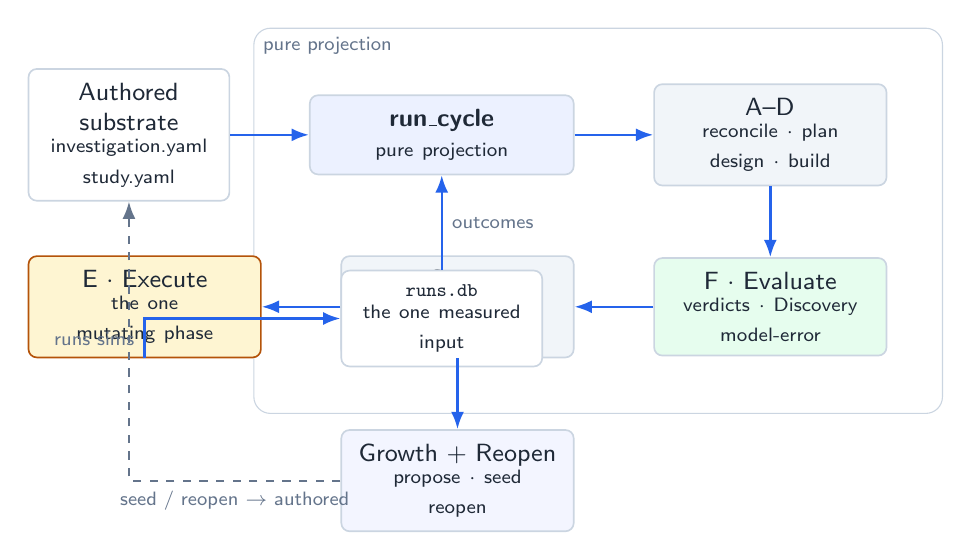
\begin{tikzpicture}[
  font=\sffamily\small,
  box/.style={rounded corners=3pt, draw=line, line width=0.6pt, fill=panel,
              text=ink, align=center, inner sep=5pt, minimum height=9mm, text width=26mm},
  core/.style={box, fill=authored!60, text width=30mm},
  eval/.style={box, fill=derived!70},
  mut/.style={box, fill=measured!80, draw=warn},
  io/.style={box, fill=white, draw=line, text width=22mm},
  flow/.style={-{Stour[length=2.2mm]}, draw=accent, line width=0.9pt},
  back/.style={-{Stour[length=2.2mm]}, draw=muted, line width=0.8pt, dashed},
  lbl/.style={text=muted, font=\sffamily\scriptsize}
]
% use a valid arrow tip name
\tikzset{flow/.style={-{Latex[length=2.2mm]}, draw=accent, line width=0.9pt}}
\tikzset{back/.style={-{Latex[length=2.2mm]}, draw=muted, line width=0.8pt, dashed}}

\node[io] (sub) {Authored substrate\\\scriptsize investigation.yaml\\\scriptsize study.yaml};
\node[core, right=10mm of sub] (core) {\textbf{run\_cycle}\\\scriptsize pure projection};
\node[box, right=10mm of core] (plan) {A--D\\\scriptsize reconcile $\cdot$ plan\\\scriptsize design $\cdot$ build};
\node[eval, below=9mm of plan] (eval) {F $\cdot$ Evaluate\\\scriptsize verdicts $\cdot$ Discovery\\\scriptsize model-error};
\node[box, left=10mm of eval] (gate) {Gates\\\scriptsize frontier $\cdot$ closure\\\scriptsize opportunities};
\node[mut, left=10mm of gate] (exec) {E $\cdot$ Execute\\\scriptsize the one\\\scriptsize mutating phase};

\node[io, below=12mm of core] (runs) {\code{\scriptsize runs.db}\\\scriptsize the one measured\\\scriptsize input};
\node[box, below=9mm of gate, fill=authored!40] (grow) {Growth + Reopen\\\scriptsize propose $\cdot$ seed\\\scriptsize reopen};

\draw[flow] (sub) -- (core);
\draw[flow] (core) -- (plan);
\draw[flow] (plan) -- (eval);
\draw[flow] (eval) -- (gate);
\draw[flow] (gate) -- (exec);
\draw[flow] (runs) -- (core) node[lbl, midway, right] {outcomes};
\draw[flow] (exec) |- (runs) node[lbl, pos=0.25, left] {runs sims};
\draw[flow] (gate) -- (grow);
\draw[back] (grow) -| (sub) node[lbl, pos=0.25, below] {seed / reopen $\rightarrow$ authored};

\begin{scope}[on background layer]
\node[fit=(core)(plan)(eval)(gate), draw=line, rounded corners=6pt,
      inner sep=7mm, label={[lbl, anchor=north west]north west:pure projection}] {};
\end{scope}
\end{tikzpicture}
\end{center}

The engine has \textbf{no single function that chains its phases}. \code{run\_cycle} is the pure
core; the lettered phases are separate functions layered on its output, each also a
\code{discover} CLI verb. The one canonical ordered step graph lives in the workbench panel;
\textbf{\code{run\_cycle} is pure}, and state changes only through the execute phase and a few
explicit write-backs.

\medskip
\noindent\textbf{The steps.} Fourteen in the panel's step graph --- thirteen pure, one mutating.

\begin{center}\small
\begin{tabular}{@{}llll@{}}
\toprule
\textbf{Step} & \textbf{Function} & \textbf{Role} & \textbf{Kind}\\
\midrule
Inputs      & \code{load\_cycle\_inputs}        & load the substrate        & pure\\
Core        & \code{run\_cycle}                 & project the whole cycle   & pure\\
A $\cdot$ Reconcile & \code{reconcile\_evidence\_state} & grade the evidence  & pure\\
B $\cdot$ Plan      & \code{plan\_candidate\_actions}   & rank the moves      & pure\\
C $\cdot$ Design    & \code{design\_discriminating\_study} & design the test  & pure\\
D $\cdot$ Build     & \code{build\_catalog} / build-model & acquire the model & pure\\
F $\cdot$ Evaluate  & \code{compare\_hypotheses}        & verdicts + Discovery & pure\\
Grading     & \code{compute\_outcomes}          & the sync that feeds the verdict & pure\\
Growth      & \code{suggest\_studies}           & propose the next studies  & pure\\
\quad $\cdot$ select & \code{select\_for\_launch}       & the autonomy gate         & pure\\
\quad $\cdot$ seed   & \code{build\_seeded\_study}      & author a run-ready study   & pure\\
\quad $\cdot$ refine & \code{refine\_study}             & deepen an existing study   & pure\\
Reopen      & \code{reconcile\_and\_reopen}     & re-enter on feedback      & pure$^\dagger$\\
E $\cdot$ Execute   & \code{advance\_cycle}             & run + change state   & \textcolor{warn}{\textbf{mut.}}\\
\bottomrule
\end{tabular}
\end{center}
{\footnotesize $^\dagger$ \code{reconcile\_and\_reopen} is a pure planner; its write happens
through the execute phase / the \code{ingest-feedback} writer. The one mutating step
(\code{advance\_cycle}) runs sandboxed in the panel --- it copies the investigation into a
throwaway workspace first, so a cycle run never touches real files.}

% ===========================================================================
\section{The data substrate --- what the cycle reads and writes}

The cycle operates on a \textbf{workspace} directory whose layout is resolved from
\code{workspace.yaml} (never hard-coded). Three artifact classes:

\begin{itemize}
\item \code{investigation.yaml} --- the investigation spec. \textbf{Authored:} \code{question},
\code{audience}, \code{studies[]}, \code{hypotheses[]}, \code{acceptance\_criteria[]},
\code{plan\_gates[]}, \code{required\_mechanisms[]}, \code{cycle\_flags}, \code{decisions\_needed},
epistemic \code{relation} tags on edges. \textbf{Cycle-written caches:} \code{resolutions[]},
\code{discoveries[]}, \code{applied\_feedback[]}, \code{lifecycle\_history}, \code{cycle\_state}
(with \code{evaluation\_snapshot}), proposal caches.
\item \code{study.yaml} --- one per member. \textbf{Authored:} \code{claim}, \code{title},
\code{question}, \code{hypothesis}, \code{behavior\_tests} (with \code{pass\_if} bands +
\code{measure}), \code{findings[]} (\code{evidence.observed}, \code{from\_test}),
\code{baseline}/variant arms, \code{observables}, \code{required\_mechanisms},
\code{parent\_studies} + relations. The \code{runs[]} list is \textbf{code-synced} from
\code{runs.db}.
\item \code{runs.db} --- SQLite, written by the simulation machinery. \textbf{The durable record
of what actually ran} --- the one measured artifact.
\end{itemize}

\paragraph{Provenance.} Throughout this map: \textbf{(H)} human-authored, \textbf{(AI)}
agent-authored (via the \code{/viva-*} skills), \textbf{(D)} derived/computed from evidence,
\textbf{(CFG)} config / schema / rollout flag. The verdict/gate/acceptance roll-ups read the
\emph{computed} outcome, not the authored one: a test that \emph{computes} fail can no longer
read ``met'' through a gate.

% ===========================================================================
\section{The stages}

Each stage: \textbf{what happens $\rightarrow$ consumes $\rightarrow$ produces $\rightarrow$
is it real?} All stages except Execute are pure and re-runnable.

\stage{Inputs --- load\_cycle\_inputs}{pure reader}
Resolves \code{investigations/<slug>/investigation.yaml}, builds the \textbf{member set} from
the spec's own \code{studies:}/\code{members:} (member-scoped --- an undeclared membership can
never pull a sibling investigation's studies into the cycle), and loads each \code{study.yaml}.
Produces \code{(inv\_path, inv\_spec, \{slug: study\_spec\})}; writes nothing. \real.

\stage{Core --- run\_cycle}{pure, no I/O}
Projects one full cycle under the merge rule. \textbf{Consumes} the authored knowledge/argument
(H/AI) merged over derived (D), per-study \code{runs[].outcomes} and \code{behavior\_tests} (D on
outcomes, H on tests), epistemic \code{relation} edges (H), and the optional evidence/viz state.
\textbf{Produces the bundle:} \code{knowledge}, \code{argument}, \code{narrative} (a
deterministic topological ordering of claims --- \emph{not} generated prose), \code{audit},
\code{gates}, \code{open\_calls}, \code{validations}, \code{suggestions}, \code{signals}
(model disagreements, anomalies), and the viz/revision proposals. The validators leave
\code{scientific\_judgment} null --- \textbf{none asserts scientific truth}. \real{} (mechanical;
quality is a function of authoring).

\stage{A --- reconcile\_evidence\_state}{pure}
Classifies each study \textbf{finding} by provenance into \code{verified} / \code{provisional} /
\code{contradicted} / \code{unsupported}, tallies a summary, and rolls each study up by its
\emph{worst} finding. \textbf{VERIFIED} requires that the cited run \emph{completed} and that
\code{observed} matches the run's \emph{computed} value within tolerance --- not merely that a
run id is registered. A study with no \code{runs.db} can never be verified. \real{} --- the one
contract (\code{registered\_run\_contract}) for ``what makes a finding run-backed.''

\stage{B --- plan\_candidate\_actions + select\_portfolio}{pure}
Recasts the frontier into classified CandidateActions (REPAIR / RESOLVE / EXTEND) with a
heuristic value score; \code{select\_portfolio} orders them (repair prereqs first, then resolve
by discrimination, then extend). \real, entirely frontier-driven --- with no hypotheses nothing
is discriminable, so the plan is all repair/extend.

\stage{C --- design\_discriminating\_study}{pure}
Returns \code{None} unless a study has a \emph{discriminable} hypothesis set ($\geq 2$ live
hypotheses predicting the same observable with \textbf{disjoint numeric bands}). Otherwise
packages the authored hypotheses into an ExperimentDesign (one arm per prediction, control arms
by naming heuristic, a pre-committed decision rule). \cond{} --- all scientific content is
authored; the function only reformats + adds control detection.

\stage{D --- build\_catalog / build-model}{pure}
Walks every study's baseline + variant arms, groups composites by path, and builds one
``component'' per composite with a token-based capability signature. Resolution
(\emph{reuse} / \emph{wrap} / \emph{build}) runs on the evidence path when a workspace root is
passed --- that route is what \emph{sources} a capability gap. A required mechanism with no
registered synonym is matched by honest token coverage, so a novel compound routes to
\textbf{BUILD} and the gap fires. In autonomous advance the \code{needs\_build} route now
resolves into a concrete immutable \textbf{ModelVersion} build (content-addressed, parent-linked;
never overwrite the model that produced prior evidence). \real.

\stage{F --- compare\_hypotheses + Discovery + model-error}{pure}
\textbf{Evaluate.} Per study, recomputes each hypothesis's support log from a quantitative source
(an observed value matching a prediction's band) and picks a \code{favored} hypothesis and a
status: \code{supported} (net${>}0$ \emph{and} VERIFIED evidence), \code{provisionally-supported},
\code{contested} (net${<}0$), \code{unresolved}, or \code{gated}. \code{model\_disagreement\_map}
surfaces multi-arm disagreement on the same observable (\emph{never averaged}); an
\emph{adjudicated} supersession is resolved history, not a live caveat.

\noindent\textbf{Discovery record (0.4.0--0.6.0).} \code{detect\_discoveries} compares the current
\code{evaluation\_snapshot} against the previous one and records a first-class \textbf{Discovery}
(scope, novelty, counterevidence, evidence refs) for every claim that \emph{flipped to a settled
outcome} (\code{supported}/\code{contested}) \textbf{on VERIFIED evidence}. Passing a gate is not
a discovery; a flip on merely provisional evidence is not one either. \textbf{(0.6.0)} the snapshot
now carries its own provenance --- a \code{schema\_version}, the \code{grader}/\code{resolver}
versions, and an \code{inputs\_hash} over the measured ledger --- and a flip diffed against a snapshot
from a \emph{different} grader/resolver or different measured inputs is \code{stale}: re-baselined,
not recorded, so a Discovery reflects new science rather than a grader bump or shifted run data.

\noindent\textbf{Model-error diagnosis (0.4.0).} On a refutation, \code{diagnose\_refutation}
emits a typed \textbf{EvidenceUpdate}: \code{revise-model} when competing model arms disagree on
the refuting observable (the model choice is implicated), else \code{revise-hypothesis} (the
model is coherent; the prediction was wrong). The diagnosis steers \emph{which} child seed the
Growth phase proposes. \real.

\stage{Grading --- compute\_outcomes}{the sync that feeds the verdict}
The reconcile sync that writes each run's \code{computed\_outcomes} block, which the roll-ups read
\emph{computed-first}. For each recorded run it grades every \code{behavior\_test} against the
run's store and writes \code{\{result, measured\_value, evaluated\_by, ...\}}. A bare-string
measure is graded through the shared \code{viva\_emitters} resolver (the engine grades
byte-identically to the workbench); a missing store degrades to the agent / needs-rerun bucket
rather than crashing. \textbf{This is the one path that reads run data} --- it is what makes a
refutation (and therefore the generative loop) fire on a \emph{computed} result, not an authored
label. \real.

\stage{Growth --- propose $\rightarrow$ select $\rightarrow$ seed $\rightarrow$ refine}{pure; the generative loop}
\textbf{Propose} (\code{suggest\_studies}) de-duplicates proposals from five sources: authored
followup proposals (H/AI), narrative-gap bridges from the audit (D), \code{decisions\_needed}
that name a member study (H, gated on a decision), and --- the \textbf{generative loop} --- a
\emph{refuted} finding auto-spawns (4) a builds-on follow-up seeded from the finding and (5) a
synthesis study folding the refutations into the next discriminating question. A refutation is a
concrete signal, so these are proposed \code{ready} and flow through the autonomy gate.
\textbf{Select} (\code{select\_for\_launch}) is a thin shim over the one \code{AutonomyPolicy}
(below): in \code{autonomous} mode every ready proposal launches; in default
\code{human\_in\_the\_loop} only approved, non-expert-gated proposals do. \textbf{Seed} (\code{build\_seeded\_study}) authors a complete, run-ready
\code{study.yaml} --- it inherits the parent's composite, observables and behavior tests (so the
child is runnable and evaluable by construction) and applies the proposal's \code{model\_change}
as the variation under test. \textbf{Refine} (\code{refine\_study}) deepens an existing study from
the engine's own signals (replicate count, low-fidelity flags). \real{} --- it proposes
\emph{where to look next} from a negative result, authors the child, and (under the autonomy
policy) promotes it to run.

\stage{Reopen --- reconcile\_and\_reopen}{pure planner; the re-entry}
Staged scientist feedback --- a compiled request on the investigation's \code{pending\_feedback[]}
--- is a first-class cycle move. It surfaces as a \code{pending\_feedback} frontier item whose op
is \textbf{reopen}; the execute phase applies it under the autonomy policy, re-opening the closed
investigation (status + verdict + \code{lifecycle\_history}) and recording the applied id in
\code{applied\_feedback[]} so it is not re-applied. \code{ingest-feedback} compiles a scientist's
reopening YAML into engine-native authored artifacts (typed actions, validated against the
schema; no prose inference). \real{} --- the structured on-ramp by which an investigation
\emph{re-enters} the cycle after a verdict.

\stage{E --- advance\_cycle}{mutating}
The phase that changes real state. Loop: reload $\rightarrow$ \code{execute\_plan} $\rightarrow$ pick
the first run-ready advance op not yet seen $\rightarrow$ check readiness $\rightarrow$ dispatch (or,
if not autonomous, record one ``would-run'' and stop). Its dispatch set widened as the loop closed:
besides running a study (\code{test}/\code{branch}) it now also \textbf{promotes a seed} to a real
study, \textbf{builds a missing mechanism}, and \textbf{reopens} on staged feedback. Every
consequential dispatch is checked against \textbf{one} \code{AutonomyPolicy} (0.4.0 unified it from
per-op gates). \real{} but \textbf{dry by default}: in the panel it runs \emph{sandboxed} on a
throwaway copy, never on real files; with no runner it reports \code{needs\_build} rather than faking
a run.

\paragraph{Supporting derivations.} Three non-blocking families ride the same projection and feed
the frontier: the \textbf{viz loop} (declared figures classified fresh / unrendered / stale /
broken, with typed proposals for uncovered gates, discriminations, and disagreements); the
\textbf{capability-gap bridge} (a required mechanism no catalog component provides $\rightarrow$ a
build-or-decline gap); and \textbf{narrative / viz-appropriateness freshness} (is a stamp stale,
is a figure shown where it belongs). They are advisory --- they inform the frontier, they do not
gate closure.

% ===========================================================================
\section{The gate system --- one engine, four views}

A single function \code{frontier()} builds the list of unresolved items; \code{closure()},
\code{next\_action()}, \code{opportunities()} and \code{execute\_plan()} are re-rankings or
filters over it. All pure and deterministic.

\subsection*{frontier() --- the one list everything reads}
An item is \emph{open} if a source raises it \textbf{and} its \code{(kind, target)} is not in the
\code{resolutions} set (the single discharge test). Each item carries a \code{priority} and an
\code{op}; the list is sorted by \code{(-priority, kind, target)}. \textbf{Closure blocks on only
three kinds} (shaded); every other kind is ``open but non-blocking.''

\begin{center}\small
\begin{tabular}{@{}rlll@{}}
\toprule
\textbf{pri} & \textbf{kind} & \textbf{op} & \textbf{blocks?}\\
\midrule
90 & \cellcolor{bad!12}unaddressed\_criterion & branch       & \blocks\\
80 & \cellcolor{bad!12}open\_challenge         & synthesize   & \blocks\\
70 & \cellcolor{bad!12}narrative\_gap          & branch       & \blocks\\
60 & open\_decision        & steer         & \nob\\
59 & pending\_feedback     & \textbf{reopen} & \nob\\
58 & revision\_proposed    & revise\_model & \nob\\
55 & stale\_validation     & revalidate    & \nob\\
50 & divergence            & reconcile     & \nob\\
48 & model\_disagreement / anomaly & revise\_model & \nob\\
47--44 & viz\_broken / viz\_missing / viz\_proposed & refine\_viz / build\_viz & \nob\\
45 & validation\_finding   & revise        & \nob\\
43 & capability\_gap       & build\_process & \nob\\
42 & pending\_gate         & test          & \nob\\
40 & open\_question        & test          & \nob\\
39 & \textbf{proposed\_study} & \textbf{seed} & \nob\\
38--35 & viz\_stale / viz\_misplaced / viz\_duplicated / viz\_untied & refine\_viz / relocate\_viz & \nob\\
\bottomrule
\end{tabular}
\end{center}
{\footnotesize \textbf{reopen} and \textbf{proposed\_study} (the seed op) are the two
loop-closing kinds. \code{viz\_untied} is behind a rollout flag, off by default.}

\subsection*{closure() --- a boolean over three kinds}
\code{closed = (no unaddressed\_criterion) and (no narrative\_gap) and (no open\_challenge)}.
No time, no threshold, no ratio. An investigation can be ``Closed'' with many open
(non-blocking) items --- closure counts only the three blocking kinds.

\subsection*{opportunities() / next\_action() $\rightarrow$ execute\_plan()}
\code{next\_action()} returns the single highest \emph{value-scored} item (re-shaped as a frontier
item), so the recommended next move and its consequence name \emph{one} item.
\code{opportunities()} re-ranks the frontier by a transparent score:
\[
\text{score} = 0.30\,\text{info} + 0.40\,\text{impact} + 0.20\,\text{enable}
+ 0.35\,\text{closure} + 0.50\,\text{discriminate} - 0.30\,\text{cost}.
\]
\code{execute\_plan()} attaches an \textbf{executor} and a \textbf{consequence tier} to each ranked
item --- it runs nothing:

\begin{center}\small
\begin{tabularx}{\textwidth}{@{}llY c@{}}
\toprule
\textbf{op} & \textbf{executor} & \textbf{consequence} & \textbf{auto?}\\
\midrule
revalidate   & snapshot-validations        & \code{safe}            & \textcolor{good}{yes}\\
test         & run-study                   & \code{simulation}      & no\\
branch       & seed-from-followup + run-study & \code{simulation+study} & no\\
seed         & promote-seed                & \code{authoring}       & no\\
reopen       & reconcile-and-reopen        & \code{reopen}          & no\\
reconcile    & set-verdict                 & \code{review}          & no\\
revise / revise\_model & act-on-validator / discover revise & \code{review} & no\\
build\_process & discover gap              & \code{review}          & no\\
build\_viz / refine\_viz (resolvable) & render-viz & \code{render}   & no\\
build\_viz / refine\_viz (stub) / relocate\_viz & discover viz & \code{review} & no\\
steer        & expert (no command)         & \code{human-only}      & no\\
synthesize   & author finding + resolve    & \code{human-only}      & no\\
\bottomrule
\end{tabularx}
\end{center}

\paragraph{AutonomyPolicy (0.4.0) --- the machine-vs-human gate.} At run time a single
\code{AutonomyPolicy} decides, per consequence tier, what may run without a human: \code{safe}
always runs; \code{simulation}/\code{simulation+study} run only in autonomous mode on a run-ready
study; \code{render} is autonomous-only and resolvable-only; \code{authoring}, \code{reopen},
\code{review} and \code{build\_process} go to an AI-decider path that records a rationale'd
resolution; \code{steer}/\code{synthesize} are always human-only. One policy now gates \emph{every}
consequential op --- the banner's ``runnable'' count and what Advance actually dispatches are the
same set by construction.

\paragraph{Discharge \& debts.} A \code{resolution \{kind, target, rationale, by?\}} removes the
matching \code{(kind, target)} from the frontier. A \code{pending\_gate} (a criterion whose study
verdict is supported but whose named behavior never ran) does not block closure but stays on the
frontier, so the debt stays visible --- distinguishing ``we concluded X'' from ``we ran the named
check for X.'' \code{capability\_gap} is deliberately excluded from the discharge kinds --- it
closes by its own build/reject lifecycle. Advisory-only: \code{diagnose()} (bottleneck
classifier) and \code{invariants()} (provenance + epistemic-separation violations) inform, they
do not gate.

% ===========================================================================
\section{What mutates vs.\ what is read-only}

A plain \code{run\_cycle} is pure. State changes only through explicit, separately-triggered
write-backs.

\begin{center}\small
\begin{tabularx}{\textwidth}{@{}llY@{}}
\toprule
\textbf{function} & \textbf{class} & \textbf{trigger}\\
\midrule
\code{run\_cycle} (+ suggest, propose\_viz) & \textsc{read-only} & every panel cycle\\
A--F (reconcile, compare, delta, discoveries) & \textsc{read-only} & panel steps A--F\\
B/C/D (plan, design, build\_catalog) & \textsc{read-only} & panel steps B/C/D\\
\code{select\_for\_launch} & \textsc{read-only} (now wired) & the \code{AutonomyPolicy} gate execute + advance consult\\
\code{build\_seeded\_study} / \code{refine\_study} & \textsc{read-only} (pure spec) & \code{-{}-write}, or autonomous \code{write\_child\_study}\\
\code{compute\_outcomes} & \textbf{writes} \code{computed\_outcomes} & reconcile sync (CLI)\\
\code{advance\_cycle} & dry by default; \textbf{writes} with \code{autonomous} & runs sims, promotes seeds, builds, reopens\\
\code{persist\_cycle} & \textbf{writes} \code{cycle\_state} + \code{discoveries} + caches & CLI cycle\\
\code{set\_verdict} / \code{record\_resolution} & \textbf{writes} verdict / resolutions & CLI, or AI-decider\\
\code{accept\_viz} / \code{accept\_capability\_gap} & \textbf{writes} viz / gap status & CLI / panel\\
\code{reconcile\_and\_reopen} & \textbf{writes} reopened spec + \code{lifecycle\_history} & CLI \code{ingest-feedback}\\
\bottomrule
\end{tabularx}
\end{center}
In the panel, the ``Apply to investigation'' button is the one surface that writes real files;
``Run continuously'' (advance) always runs \textbf{sandboxed}. Human-only (steer/synthesize) items
are never auto-resolved.

% ===========================================================================
\section{Authored vs.\ derived --- the consolidated matrix}

Left = the authored substrate (the only true inputs); right = everything the engine computes from
it. The one \emph{measured} input is the simulation run.

\begin{center}\small
\begin{tabularx}{\textwidth}{@{}>{\columncolor{authored!40}}Y >{\columncolor{derived!40}}Y@{}}
\toprule
\textbf{authored by a human or AI} & \textbf{derived mechanically by the engine}\\
\midrule
Study \textbf{claim} sentence & claim verdict (from run outcomes), \code{diverges} flag\\
Behavior tests + \code{pass\_if} + \code{measure} & per-test PASS/FAIL $\rightarrow$ study verdict\\
Hypotheses + numeric \code{predictions} & support log, favored, designs, disagreements\\
Acceptance criteria & \code{unaddressed\_criterion} / \code{pending\_gate} items\\
Epistemic \code{relation} tags & argument edges, narrative order, audit gaps\\
\code{plan\_gates} (synthesis spine) & rolled-up gate verdicts\\
\code{decisions\_needed} & \code{open\_decision} items, steer actions, enable score\\
Findings \code{statement} + \code{from\_test} & verified / provisional / contradicted classification\\
\code{required\_mechanisms} contract & capability-gap proposals + build\_process items\\
\code{followup\_proposals} / \code{model\_change} & proposal list, candidate actions, portfolio order\\
A \textbf{refuted} finding (its evidence) & \textbf{Discovery} records; \textbf{EvidenceUpdate} (revise-model / -hypothesis)\\
Scientist \textbf{reopening feedback} & \code{reopen} op; re-entered spec + \code{lifecycle\_history}\\
A decision's resolution (rationale) & frontier discharge; executive renewal\\
The \textbf{simulation itself} (external runner) & run records $\rightarrow$ run ids, outcomes, evidence status\\
\bottomrule
\end{tabularx}
\end{center}
The engine's value is that it keeps the right column consistent with --- and always re-derivable
from --- the left (``authored wins, derived fills''), and explicitly refuses to fabricate verdicts
or resolve human-only decisions.

% ===========================================================================
\section{What is real vs.\ conditional vs.\ unwired}

\real{} = computes genuinely over real data. \cond{} = real only when the right fields are
authored. \unwired{} = engine-complete but nothing in the product calls or executes it.

\begin{center}\small
\begin{tabularx}{\textwidth}{@{}l l Y@{}}
\toprule
\textbf{stage / family} & \textbf{grade} & \textbf{why}\\
\midrule
Inputs, Core, A, B & \real & pure readers / projection over real YAML + run data\\
Grading (\code{compute\_outcomes}) & \real & the one run-data path; feeds the verdict computed-first\\
F $\cdot$ Evaluate & \cond & \code{unresolved} without authored hypotheses + predictions\\
F $\cdot$ Discovery + model-error & \real & fire on a \emph{computed} refutation; 0 discoveries if a study has no hypothesis snapshot\\
D $\cdot$ Model build & \real & novel mechanisms route to BUILD; autonomous advance builds a real ModelVersion\\
C $\cdot$ Design & \cond & \code{None} without $\geq 2$ disjoint-band hypotheses\\
Growth (propose / generative loop) & \real & a refuted finding proposes \emph{and} (if authorized) runs the next study\\
Growth $\cdot$ select / AutonomyPolicy & \real & one policy gates every consequential op; drives promotion\\
Growth $\cdot$ seed / refine & \real & pure spec; autonomous write-back via \code{write\_child\_study}\\
E $\cdot$ Execute / advance & \real, dry by default & sandboxed in the panel; one AutonomyPolicy gates every op\\
Reopen & \real & structured re-entry on staged feedback; typed, schema-validated\\
Gate system & \real & deterministic; three blocking kinds; value-ranked next action\\
Self-contained CLI + linkage & \real & report / lint / observations / linkage as headless \code{discover} verbs (0.4.1--0.5.0)\\
Versioned evidence snapshot & \real & snapshot provenance + stale-Discovery gate (0.6.0)\\
Viz loop & \real & engine + full panel wiring (propose / build / declare / accept)\\
capability-gap bridge & \cond & engine-complete; no workbench endpoint yet\\
viz-appropriateness & thin & items only; the relocate op has no executor yet\\
\bottomrule
\end{tabularx}
\end{center}

\paragraph{Honest edges.} Two things are defined-but-unwired, and worth naming rather than hiding:
the \textbf{capability-gap bridge} is engine-complete but has no workbench endpoint (it surfaces as an
unlabeled row), and \textbf{viz-appropriateness} emits items but its relocate op has no executor. The
Growth autonomy gate, by contrast, is \emph{now wired} --- one \code{AutonomyPolicy} drives promotion
in \code{execute\_action} and \code{advance\_cycle}. Everything else on the spine --- load, project,
reconcile, grade, evaluate, record, and the explicit write-backs --- operates on real artifacts, and
the loop closes end to end: a refuted finding proposes \emph{and runs} the next study, a
settled+verified verdict records a discovery (re-baselined if the evidence snapshot is stale), and
scientist feedback re-enters through reopen.

\vfill
\begin{center}\footnotesize\color{muted}
discovery-engine 0.6.0 \;$\cdot$\; derive-first \;$\cdot$\; one measured input \;$\cdot$\; the loop closes
\end{center}

\end{document}
